\subsection{Amministratore}

\subsubsection{Panoramica Amministratore}
\begin{figure}[H]
\centering
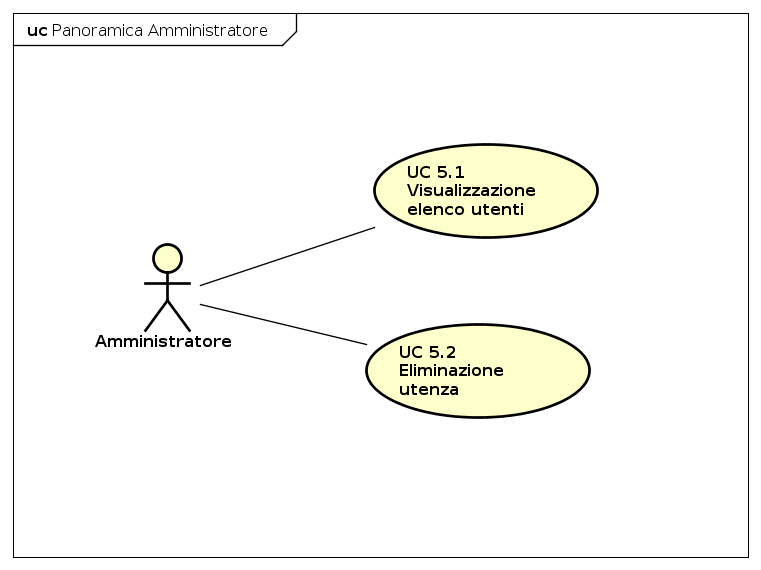
\includegraphics[width=17cm, height=10cm]{img/PanoramicaAmministratore.png} 
\caption{Panoramica Amministratore}
\end{figure}


\subsubsection{UC 5.1 - Visualizzazione della propria dashboard}


\begin{figure}[H]
\centering
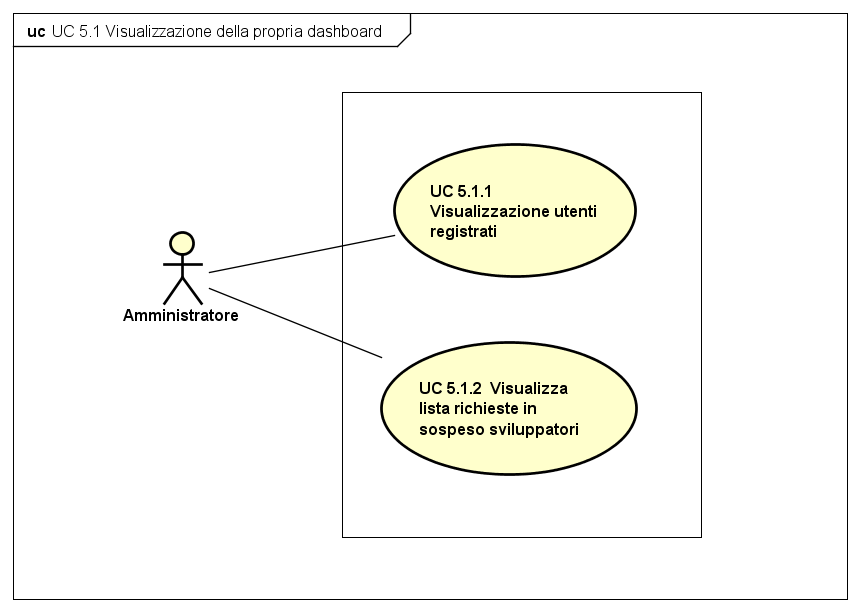
\includegraphics[width=17cm, height=10cm]{img/UC51.png} 
\caption{Caso d'uso UC 5.1}
\end{figure}


\begin{itemize}
\item[•] \textbf{Attore}: Amministratore; 
\item[•] \textbf{Descrizione}: L'amministratore accede alla propria dashboard personale e può effettuare modifiche al sistema;
\item[•] \textbf{Precondizione}: Il sistema offre la possibilità di accedere alla propria dashboard;
\item[•] \textbf{Postcondizione}: L'amministratore è all'interno della sua dashboard;
\item[•] \textbf{Flusso degli eventi}:

\begin{enumerate}
\item UC 5.1.1 Visualizzazione utenti registrati;
\item UC 5.1.2 Visualizza lista richieste in sospeso sviluppatori.
\end{enumerate}

\end{itemize}
\subsubsection{UC 5.1.1 - Visualizzazione utenti registrati}

\begin{figure}[H]
\centering
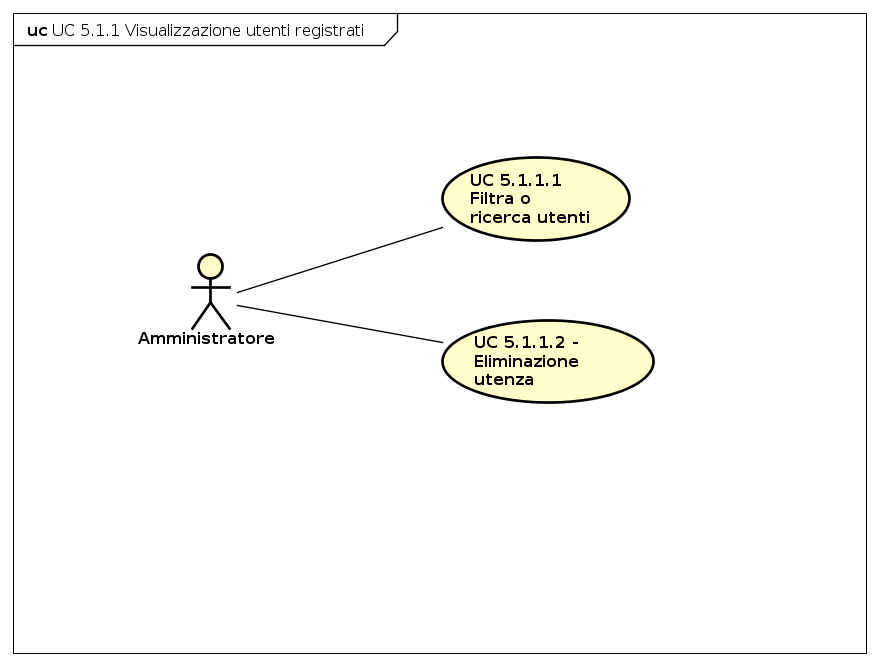
\includegraphics[width=17cm, height=10cm]{img/UC511.png} 
\caption{Caso d'uso UC 5.1.1}
\end{figure}


\begin{itemize}
\item[•] \textbf{Attore}: Amministratore;

\item[•] \textbf{Descrizione}: L'amministratore visualizza l'elenco degli utenti registrati nel sistema;

\item[•] \textbf{Precondizione}: L'amministratore si è autenticato nel sistema e visualizza la propria dashboard;

\item[•] \textbf{Postcondizione}: L'amministratore visualizza la lista di utenti registrati al sistema; 

\item[•] \textbf{Flusso degli eventi}:

% L'amministratore accede alla pagina contenente l'elenco degli utenti e visualizza i dati degli utenti. 

\begin{enumerate}

\item UC 5.1.1.1 - Filtra o ricerca utenti;
\item UC 5.1.1.2 - Eliminazione utenza.

\end{enumerate}
\end{itemize}

\subsubsection{UC 5.1.1.1 - Filtra o ricerca utenti}
\begin{itemize}

\item[•] \textbf{Attore}: Amministratore;
\item[•] \textbf{Descrizione}: L'amministratore ha la possibilità di ricercare gli utenti a partire dal loro nome o dalla loro tipologia di utenza;
\item[•] \textbf{Precondizione}: Il sistema offre la possibilità di filtrare o cercare gli utenti a seconda del loro nome o della loro tipologia di utenza;
\item[•] \textbf{Postcondizione}: Il sistema visualizza gli utenti selezionati.

\end{itemize}
%%%%%%%% Dubbio su estensione, io metterei che l'amministratore può cancellare l'utente che ha trovato con la ricerca %%%%%%%%%%%%%%%%

\subsubsection{UC 5.1.1.2 - Eliminazione utenza}

% Immagine tolta percè il caso d'uso ha solo operazioni atomiche 

%\begin{figure}[H]
%\centering
%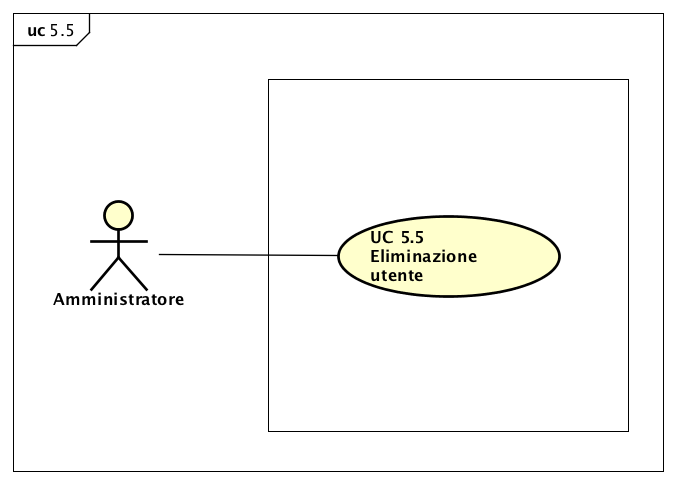
\includegraphics[width=17cm, height=10cm]{img/UC55.png} 
%\caption{Caso d'uso UC5.2}
%\end{figure}

\begin{itemize}
\item[•] \textbf{Attore}: Amministratore;
\item[•] \textbf{Descrizione}: L'amministratore elimina un'utenza dal sistema;
\item[•] \textbf{Precondizione}: L'amministratore \`{e} autenticato e visualizza l'elenco degli utenti registrati nel sistema ed ha selezionato un utente da eliminare;
\item[•] \textbf{Postcondizione}: L'amministratore ha eliminato l'utenza dal sistema; 
\item[•] \textbf{Flusso degli eventi}:

\begin{enumerate}
%\item Selezione utente;
\item Conferma eliminazione utente;
\item Annulla eliminazione.
\end{enumerate}
\end{itemize}


\subsubsection{UC 5.1.2 - Visualizza lista richieste in sospeso sviluppatori}
\begin{itemize}

\item[•] \textbf{Attore}: Amministratore;
\item[•] \textbf{Descrizione}: L'amministratore visualizza tutti gli utenti che si vogliono registrare come sviluppatori nel sistema e può accettare o no l'iscrizione;
\item[•] \textbf{Precondizione}: Il sistema offre la possibilità di visualizzare la lista degli utenti che si vogliono registrare come sviluppatori;
\item[•] \textbf{Postcondizione}: L'amministratore visualizza la lista delle richieste in sospeso;
\item[•] \textbf{Flusso degli eventi}:
\begin{enumerate}
\item Accetta sviluppatore;
\item Rifiuta sviluppatore.
\end{enumerate}

\end{itemize}
%\subsubsection{UC5.2 - Visualizzazione elenco richieste}
%
%\begin{figure}[H]
%\centering
%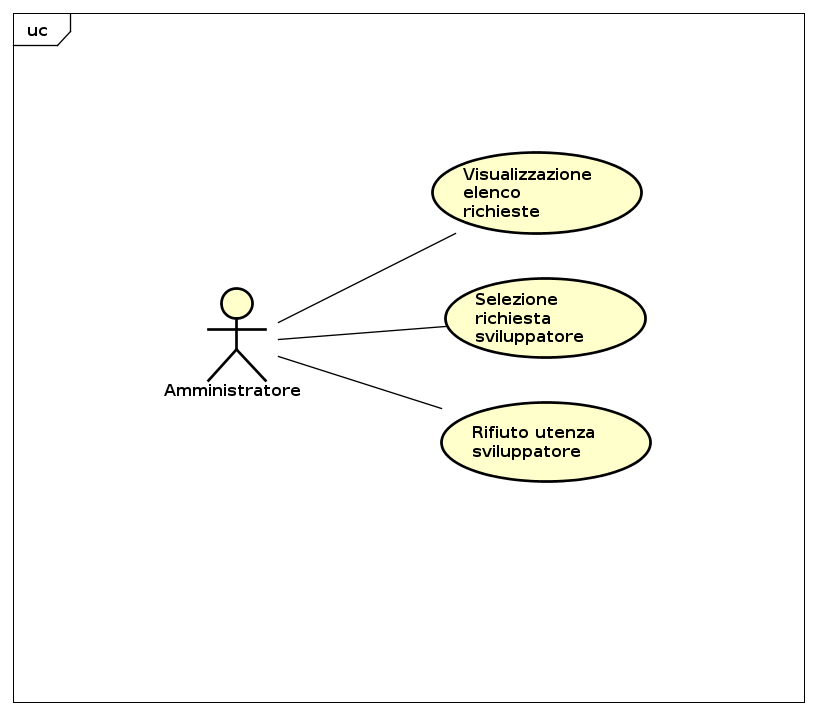
\includegraphics[height=9cm, width=17cm]{img/UC52.png} 
%\caption{Caso d'uso UC5.2}
%\end{figure}
%
%
%\begin{itemize}

%\end{itemize}
%\item[•] \textbf{Attore}: Amministratore;
%
%\item[•] \textbf{Descrizione}: L'amministratore visualizza l'elenco delle richieste provenienti da utenti che intendono registrarsi nel sistema come sviluppatori;
%
%\item[•] \textbf{Precondizione}: L'amministratore si è autenticato nel sistema e visualizza la propria dashboard;
%
%\item[•] \textbf{Postcondizione}: L'amministratore visualizza l'elenco delle richieste effettuate che devono ancora essere gestite;
%
%\item[•] \textbf{Flusso degli eventi}: L'amministratore accede alla pagina contenete l'elenco delle richieste che necessitano di un intervento da parte dell'amministratore.
%\end{itemize}
%
%\subsubsection{UC5.3 - Approvazione registrazione}
%\begin{figure}[H]
%\centering
%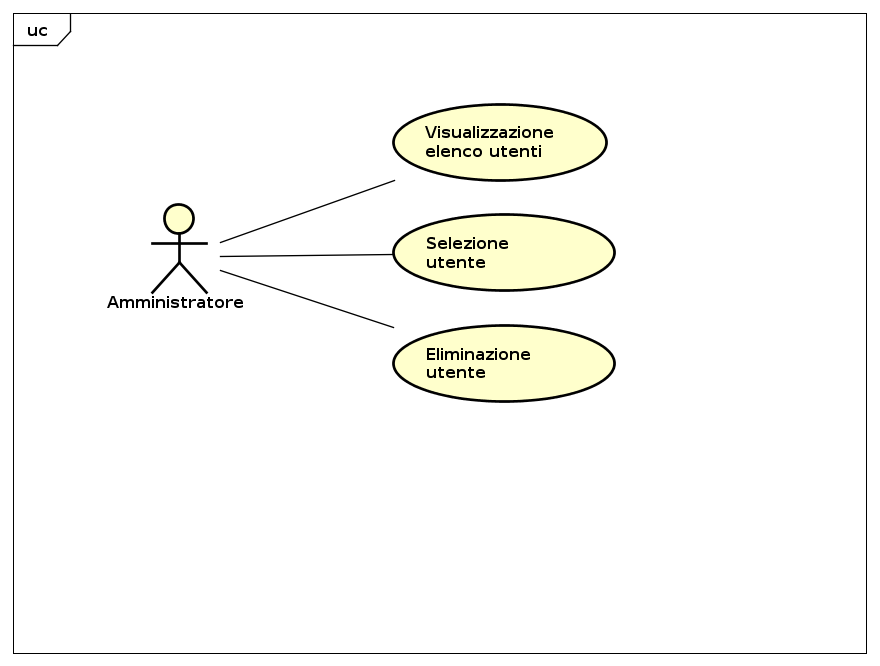
\includegraphics[width=17cm, height=9cm]{img/UC53.png} 
%\caption{Caso d'uso UC5.3}
%\end{figure}
%
%\begin{itemize}
%\item[•] \textbf{Attore}: Amministratore;
%
%\item[•] \textbf{Descrizione}: L'amministratore approva la richiesta di registrazione da parte dello sviluppatore;
%
%\item[•] \textbf{Precondizione}: Lo sviluppatore ha effettuato richiesta di registrazione, l'amministratore visualizza le richieste di registrazione da parte degli sviluppatori che desiderano accedere ai dati della piattaforma;
%
%\item[•] \textbf{Postcondizione}: L'amministratore approva la richiesta di registrazione sviluppatore che quindi può registrarsi;
%
%\item[•] \textbf{Flusso degli eventi}:
%
%\begin{enumerate}
%
%\item UC 5.2 - Visualizzazione elenco richieste;
%
%\item Selezione richiesta sviluppatore;
%
%\item Approvazione richiesta sviluppatore.
%
%\end{enumerate}
%
%\end{itemize}
%
%
%\subsubsection{UC5.4 - Rifiuto registrazione}
%
%\begin{figure}[H]
%\centering
%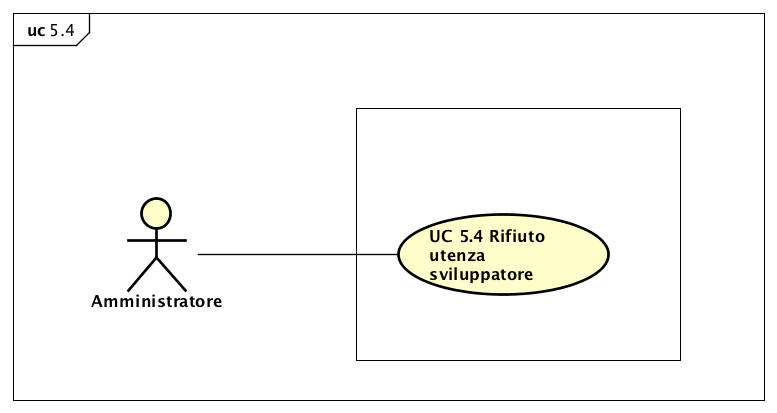
\includegraphics[width=17cm, height=9cm]{img/UC54.png} 
%\caption{Caso d'uso UC5.4}
%\end{figure}
%
%
%\begin{itemize}
%\item[•] \textbf{Attore}: Amministratore;
%
%\item[•] \textbf{Descrizione}: L’amministratore rifiuta la richiesta di registrazione da parte dello sviluppatore;
%
%\item[•] \textbf{Precondizione}: Lo sviluppatore ha richiesto l'approvazione, l'amministratore visualizza la richiesta di registrazione da parte dello sviluppatore che desidera accedere ai dati della piattaforma;
%
%\item[•] \textbf{Postcondizione}: L'amministratore rifiuta la richiesta di registrazione dello sviluppatore;
%
%\item[•] \textbf{Flusso degli eventi}:
%
%\begin{enumerate}
%
%\item UC 5.2 - Visualizzazione elenco richieste;
%
%\item Selezione richiesta sviluppatore;
%
%\item Rifiuto utenza sviluppatore.
%
%\end{enumerate}
%\end{itemize}


% in seguito a discussione con Damien è stato tolto 10/01/2019

